\begin{center}\large\textbf{Readings: 17.1-17.8}\\
\normalsize \end{center}
\large ~\hrulefill
~\\

Models with both fixed and random factors are called \textbf{Mixed Models}.  Let's do some practice picking out fixed and random factors along with nested and crossed design.\\

\textbf{Two-factor designs examples (some repeated from previous notes)}
\begin{enumerate}
\item Entomologist records energy expended ($y$) by $N=27$ honeybees
\begin{itemize}
\item at three TEMPERATURES ($20,30,40^o C$)
\item consuming three levels of SUCROSE $(20\%,40\%,60\%)$ 
\end{itemize}
 
\begin{large}
\begin{center}
\begin{tabular}{|cc|ccc|}  \hline
Temp & Suc & \multicolumn{3}{c|}{Sample} \\ \hline
   20 & 20 & 3.1 & 3.7 & 4.7 \\
   20 & 40 & 5.5 & 6.7 & 7.3 \\
   20 & 60 & 7.9 & 9.2 & 9.3 \\
   30 & 20 & 6 & 6.9 & 7.5 \\
   30 & 40 & 11.5 & 12.9 & 13.4 \\
   30 & 60 & 17.5 & 15.8 & 14.7 \\
   40 & 20 & 7.7 & 8.3 & 9.5 \\
   40 & 40 & 15.7 & 14.3 & 15.9 \\
   40 & 60 & 19.1 & 18.0 & 19.9 \\ \hline
\end{tabular}
\end{center}
\end{large}

\begin{itemize}
\item First factor: \textcolor{red}{Temp}
\item Second factor: \textcolor{red}{Sucrose}
\item Fixed or random? \textcolor{red}{Both fixed}
\item Crossed or nested? \textcolor{red}{Crossed}
\item Model:  
%$Y_{ijk} = \mu + \hspace{3in} + E_{ijk}$
\textcolor{red}{$Y_{ijk} = \mu + \alpha_i+\beta_j+(\alpha\beta)_{ij} + E_{ijk}$}
\end{itemize}


\item Experiment to study effect of drug and method of administration on fasting blood sugar in a random sample of $N=18$ diabetic patients.
\begin{large}
\begin{center}
\begin{tabular}{llccccc}
Drug ($i$) & Type of Administration $(j)$ & Mean $\bar{y}_{j(i)}$ & Variance $s_{j(i)}^2$ \\ \hline
$(i=1)$ Brand I tablet & $(j=1)30 mg \times 1$ & 15.7 & 6.3 \\
& $(j=2)15 mg \times 2$ & 19.7 & 9.3 \\
$(i=2)$ Brand II tablet & $(j=1)20 mg \times 1$ & 20 & 1 \\
& $(j=2)10 mg \times 2$ & 17.3 & 6.3 \\
$(i=3)$ Insulin injection & $(j=1)$ before breakfast  & 28  & 4 \\
& $(j=2)$ before supper & 33 & 9 \\ \hline
\end{tabular}
\end{center}
\end{large}

\begin{itemize}
\item First factor:\textcolor{red}{Drug}
\item Second factor:\textcolor{red}{Admin}
\item Fixed or random?\textcolor{red}{Both fixed}
\item Crossed or nested?\textcolor{red}{Nested, Admin(Drug)}
\item Model: %$Y_{ijk} = \mu + \hspace{3in} + E_{ijk}$
\textcolor{red}{$Y_{ijk} = \mu + \alpha_i+\beta_{(i)j} + E_{ijk}$}
\end{itemize}

\item An experiment is conducted to determine variability among laboratories (interlaboratory differences) in their assessment of bacterial 
concentration in milk after pasteurization.   Milk w/ various degrees of contamination was tested by randomly drawing four samples of milk from a collection of cartons at various stages of spoilage.  Each of the four samples was split into 10 parts and two were sent to each of the 5 laboratories.  $Y$ is colony-forming units/$\mu l$.  Labs think they're receiving 8 independent samples.
\begin{large}
\begin{center}
\begin{tabular}{c|cccc}
& \multicolumn{4}{c}{Sample} \\
Lab & 1 & 2 & 3 & 4 \\ \hline 
1 & 2200 & 3000 & 210 & 270 \\
  & 2200 & 2900 & 200 & 260 \\
2 & 2600 & 3600 & 290 & 360 \\
  & 2500 & 3500 & 240 & 380 \\
3 & 1900 & 2500 & 160 & 230 \\
  & 2100 & 2200 & 200 & 230 \\
4 & 2600 & 2800 & 330 & 350 \\
  & 4300 & 1800 & 340 & 290 \\
5 & 4000 & 4800 & 370 & 500 \\
  & 3900 & 4800 & 340 & 480 \\  
\end{tabular}
\end{center}
\end{large}

\begin{itemize}
\item First factor:\textcolor{red}{Lab}
\item Second factor:\textcolor{red}{Sample}
\item Fixed or random?\textcolor{red}{Both random}
\item Crossed or nested?\textcolor{red}{Crossed}
\item Model:  %$Y_{ijk} = \mu + \hspace{3in} + E_{ijk}$
\textcolor{red}{$Y_{ijk} = \mu + A_i+B_j+(AB)_{ij} + E_{ijk}$}
\end{itemize}

\item An expt measures {\em Campylobacter} counts in $N=120$ chickens in a processing plant, at four locations, over three days.  Means (std) for $n=10$ chickens sampled at each location tabulated below:
\begin{itemize}
\item Student visits plant on three random sampled winter days.
\item On each day he samples $n=10$ chickens at each of four locations, or sites, along the washing line: (before first washer, after 3rd washer, after microbial rinse, after chill tank)
\end{itemize}
\begin{center}
\begin{large}
\begin{tabular}{c|cccc}
& \multicolumn{4}{c}{Location} \\
& Before & After & After & After \\
Day & Washer & Washer & mic. rinse & chill tank \\ \hline
 1       &       70070.00      &      48310.00      &      12020.00      &      11790.00 \\
         &      (79034.49)     &     (34166.80)     &      (3807.24)     &      (7832.05)\\
 2       &       75890.00      &      52020.00      &       8090.00      &       8690.00 \\
         &      (74551.32)     &     (17686.27)     &      (4848.01)     &      (5526.19) \\
 3       &       95260.00      &      33170.00      &       6200.00      &       8370.00 \\
         &      (03176.00)     &     (22259.08)     &      (5028.81)     &      (5720.15) \\ \hline
\multicolumn{5}{c}{Data courtesy of Michael Bashor, General Mills } \\
\end{tabular}
\end{large}
\end{center}

\begin{itemize}
\item First factor:\textcolor{red}{Location}
\item Second factor:\textcolor{red}{Day}
\item Fixed or random?\textcolor{red}{Loacation fixed, Day random}
\item Crossed or nested?\textcolor{red}{Crossed}
\item Model:  
%$Y_{ijk} = \mu + \hspace{3in} + E_{ijk}$
\textcolor{red}{$Y_{ijk} = \mu + \alpha_i+B_j+(\alpha B)_{ij} + E_{ijk}$}
\end{itemize}

\item An experiment to assess the variability of a particular acid among plants was done.  Many plants were planted and 4 were randomly selected.  Then three leaves were selected from each plant to be measured.
\begin{large}
\begin{center}
\begin{tabular}{c|ccc|ccc|ccc|ccc}
Plant $i$ & \multicolumn{3}{c}{1} & \multicolumn{3}{c}{2} & \multicolumn{3}{c}{3} & \multicolumn{3}{c}{4}  \\ \hline
Leaf $j$ & 1 & 2 & 3 & 1 & 2 & 3 & 1 & 2 & 3 & 1 & 2 & 3 \\ \hline
$k=1$ & 11.2 & 16.5 & 18.3 & 14.1 & 19.0 & 11.9 & 15.3 & 19.5 & 16.5 & 7.3 & 8.9 & 11.3 \\
$k=2$ & 11.6 & 16.8 & 18.7 & 13.8 & 18.5 & 12.4 & 15.9 & 20.1 & 17.2 & 7.8 & 9.4 & 10.9 \\
$k=3$ & 12.0 & 16.1 & 19.0 & 14.2 & 18.2 & 12.0 & 16.0 & 19.3 & 16.9 & 7.0 & 9.3 & 10.5 \\ \hline
\multicolumn{12}{l}{Data from Neter, et al (1996)}
\end{tabular}
\end{center}
\end{large}

\begin{itemize}
\item First factor:\textcolor{red}{Plant}
\item Second factor:\textcolor{red}{Leaf}
\item Fixed or random?\textcolor{red}{Both random}
\item Crossed or nested?\textcolor{red}{Nested, Leaf(Plant)}
\item Model:  
%$Y_{ijk} = \mu + \hspace{3in} + E_{ijk}$
\textcolor{red}{$Y_{ijk} = \mu + A_i+B_{(i)j}+ E_{ijk}$}
\end{itemize}


\item 5 treatments of light intensity were assigned randomly to 10 pots of plants.  Each pot had two seedlings per pot.  For each seedling the plant height was measured for a total of 20 measurements. (See Table 14.2 from Rao.)
\begin{small}
\begin{center}
\begin{tabular}{cc|cc}
Treatment & Pot & Seedling 1 & Seedling 2 \\ \hline
1          &       1       &      32.94      &      35.98 \\
1          &       2       &      34.76      &      32.40 \\
2          &       1       &      30.55      &      32.64 \\
2          &       2       &      32.37      &      32.04 \\
3          &       1       &      31.23      &      31.09 \\
3          &       2       &      30.62      &      30.42 \\
4          &       1       &      34.41      &      34.88 \\
4          &       2       &      34.07      &      33.87 \\
5          &       1       &      35.61      &      35.00 \\
5          &       2       &      33.65      &      32.91 \\ \hline
\end{tabular}
\end{center}
\end{small}

\begin{itemize}
\item First factor:\textcolor{red}{Treatment}
\item Second factor:\textcolor{red}{Pot}
\item Fixed or random?\textcolor{red}{Treatment fixed, Pot random}
\item Crossed or nested?\textcolor{red}{Nested, Plot(Treatment)}
\item Model: %$Y_{ijk} = \mu + \hspace{3in} + E_{ijk}$
\textcolor{red}{$Y_{ijk} = \mu + \alpha_i+B_{(i)j} + E_{ijk}$}
\end{itemize}
\end{enumerate}

\textbf{Recap:  Six types of two-factor models possible with fixed and/or random effects that are either crossed or nested.}
\begin{center}
\begin{tabular}{l|ccl|l}
Experiment Number & && Model & Identifier\\
%\underbar{~~~~~} 
\textcolor{red}{3}
& $Y_{ijk}$&=&$\mu + A_i + B_j + (AB)_{ij} + E_{ijk}$  & \mbox{crossed/random} \\
%\underbar{~~~~~} 
\textcolor{red}{2}
& $Y_{ijk}$&=&$\mu + \alpha_i + \beta_{(i)j} + E_{ijk}$ &  \mbox{nested/fixed} \\
%\underbar{~~~~~} 
\textcolor{red}{5}
& $Y_{ijk}$&=&$\mu + A_i + B_{(i)j} + E_{ijk}$  & \mbox{nested/random} \\
%\underbar{~~~~~} 
\textcolor{red}{4}
& $Y_{ijk}$&=&$\mu + \alpha_i + B_j + (\alpha B)_{ij} + E_{ijk}$  & \mbox{crossed/mixed} \\
%\underbar{~~~~~} 
\textcolor{red}{6}
& $Y_{ijk}$&=&$\mu + \alpha_i + B_{(i)j} + E_{ijk}$  & \mbox{nested/mixed} \\
%\underbar{~~~~~} 
\textcolor{red}{1}
& $Y_{ijk}$&=&$\mu + \alpha_i + \beta_j + (\alpha\beta)_{ij} + E_{ijk}$ & \mbox{crossed/fixed} \\
\end{tabular}
\end{center}

\begin{itemize}
\item GREEK symbols parameterize FIXED, unknown treatment means 
\item CAPITAL letters represent RANDOM effects
\end{itemize}
In the models above there are many constraints
\begin{itemize}
\item for first model above, $A_i,B_i,(AB)_{ij}$ are all independent
\item for second model above, $\sum \alpha_i = \sum_j \beta_{(i)j} \equiv  0$
\item for third model above, $A_i,B_{(i)j}$ are all independent
\item for fourth model above, $\sum \alpha_i=0$ and $B_j,(\alpha B)_{ij}$ are all independent
\item for fifth model above, $\sum \alpha_i=0$ 
\item for sixth model above, $\sum \alpha_i = \sum \beta_j = \sum_i (\alpha\beta)_{ij} = \sum_j (\alpha\beta)_{ij} \equiv 0$
\end{itemize}

\newpage

One method for making inference in Mixed Models is to equate mean squares to find appropriate tests.  Below are tables of mean squares for these different models:\\~\\
\textbf{Tables of expected means squares (EMS):}\\
When factors $A$ and $B$ are CROSSED, and no sum-to-zero assumptions are made on random effects, expected means associated with sums of squares are given in the table below:
\begin{large}
\begin{center}
\begin{tabular}{ccccc}
Source & $df$ & $A,B$ fixed & $A,B$ random & $A$ fixed $B$ random \\ \hline
$A$ & $a-1$ & $\sigma^2 + nb \psi_A^2$ & $\sigma^2 + nb \sigma_A^2 + n\sigma_{AB}^2$ & $\sigma^2 + nb \psi_A^2 + n\sigma_{\alpha B}^2$ \\
$B$ & $b-1$ & $\sigma^2 + na \psi_B^2$ & $\sigma^2 + na \sigma_B^2 + n\sigma_{AB}^2$ & $\sigma^2 + na \sigma_B^2 + n\sigma_{\alpha B}^2$ \\
$AB$ & $(a-1)(b-1)$ & $\sigma^2 + n \psi_{AB}^2$ & $\sigma^2 + n\sigma_{AB}^2$ & $\sigma^2 + n\sigma_{\alpha B}^2$\\
Error & $ab(n-1)$ & $\sigma^2$ & $\sigma^2$ & $\sigma^2$ \\ \hline
\end{tabular} 
\end{center} 
\end{large}

When factor $B$ is NESTED in factor $A$, expected means associated with sums of squares are given in the table below:
\begin{large}
\begin{center}
\begin{tabular}{ccccc}
Source & $df$ & $A,B$ fixed & $A,B$ random & $A$ fixed $B$ random \\ \hline
$A$ & $a-1$ & $\sigma^2 + nb \psi_A^2$ & $\sigma^2 + nb \sigma_A^2 + n\sigma_{B(A)}^2$ & $\sigma^2 + nb \psi_A^2 + n\sigma_{B(A)}^2$ \\
$B(A)$ & $a(b-1)$ & $\sigma^2 + n \psi_{B(A)}^2$ & $\sigma^2 + n \sigma_{B(A)}^2$ & $\sigma^2 + n \sigma_{B(A)}^2$ \\
Error & $ab(n-1)$ & $\sigma^2$ & $\sigma^2$ & $\sigma^2$ \\ \hline
\end{tabular} 
\end{center} 
\end{large}
where $\psi^2$ and $\sigma^2$ values are defined below.

\begin{eqnarray*}
\psi_A^2 & = & \frac{1}{a-1} \sum_1^a \alpha_i^2 \ \ \ \mbox{ effect size of factor } A\\
\psi_B^2 & = & \frac{1}{b-1} \sum_1^b \beta_i^2 \ \ \ \ \mbox{ effect size of factor } B\\
\psi_{AB}^2 & = & \frac{1}{(a-1)(b-1)} \sum_{i=1}^a\sum_{j=1}^b (\alpha\beta)_{ij}^2 \ \mbox{ effect size of interaction } \\
\psi_{B(A)}^2 & = & \frac{1}{a(b-1)} \sum_{i=1}^a\sum_{j=1}^b \beta_{(i)j}^2 \ \ \ \mbox{ effect size of factor } B\\
\sigma_A^2 & = & \Var(A_i) \ \ \ \mbox{ variance component for factor } A\\
\\
\sigma_B^2 & = & \Var(B_i) \ \ \ \mbox{ variance component for factor } B\\
\\
\sigma_{AB}^2 & = & \Var((AB)_{ij}) \ \ \ \mbox{ variance component for interaction } \\
\\
\sigma_{B(A)}^2 & = & \Var(B_{(i)j})\ \ \ \mbox{ variance component for factor }B \\
\\
\sigma^2 & = & \Var(E_{ijk)})\ \ \ \mbox{ error variance} 
\end{eqnarray*} 

We can use these expected mean squares to determine tests for effects.\\~\\
Example: For A fixed, B random in a crossed experiment
$$E(MS(A))=\sigma^2 + nb \psi_A^2 + n\sigma_{\alpha B}^2$$
$$E(MS(AB))=\sigma^2 + n\sigma_{\alpha B}^2$$
Thus, a test for the effect of A can be derived as 
$$F=MS(A)/MS(AB)~~~~vs~~~~F(\alpha, a-1, (a-1)(b-1))$$
If $H_0: \alpha_i=0$ for all $i$ is true, then this F should be approximately 1. \\
If $H_A:$ at least 1 $\alpha_i\neq 0$ is true, then this F should be larger than 1.\\~\\
To determine if we are far enough from 1 we should compare to the appropriate F critical value.\\~\\

\textbf{Help with computing expected mean squares for balanced designs (without sum-to-zero assumptions on random effects)}
\begin{enumerate}
\item If a factor $X$ with index $i$ is random then $EMS(X)$ is a linear combo of $\sigma^2$ and varcomps for all random effects containing index $i$.  Coefficients for varcomps are limits of indexes NOT listed (summed over) in random effects.
\item If a factor $X$ is fixed.  Treat it like it is random and then just replace the varcomp for $X$ with the effect size, $\psi_X^2$. 
\end{enumerate} 

\textcolor{red}{ex: Suppose you have 3 factors with factor B fixed and factors A and C random, factors crossed.  To find the expected mean squares:
$$Y_{ijkl}=\mu+A_i+\beta_j+C_k+(A\beta)_{ij}+(AC)_{ik}+(\beta C)_{jk}+(A\beta C)_{ijk}+E_{ijkl}$$
Then 
$$E(MS(B))= \sigma^2+n\sigma^2_{A\beta C}+na\sigma^2_{\beta C}+nc\sigma^2_{A\beta}+nac\psi^2_{\beta}$$
$$E(MS(ABC))=\sigma^2+n\sigma^2_{A\beta C}$$
$$E(MS(A))= \sigma^2+n\sigma^2_{A\beta C}+nb\sigma^2_{AC}+nc\sigma^2_{A\beta}+nbc\sigma^2_{A}$$
Sometimes you have to solve for things to get correct error term.  Error term to use for testing of factor B's importance is 
$$MS(AB)+MS(BC)-MS(ABC)$$
}

\newpage

\textbf{Analysis of milk example - $F$-tests and estimating variance components.} \\
Recall: We have crossed random factors.  
\begin{enumerate}
\item To test for interaction effect, use $F_{AB}=\frac{MS[AB]}{MS[E]}$ vs $F(\alpha,(a-1)(b-1),ab(n-1))$
\item To test for main effect of A, use $F_{A}=\frac{MS[A]}{MS[AB]}$ vs $F(\alpha,a-1,(a-1)(b-1))$
\item To test for main effect of B, use $F_{B}=\frac{MS[B]}{MS[AB]}$ vs $F(\alpha,b-1,(a-1)(b-1))$
\end{enumerate}
Note the departure from fixed effects analysis, where $MS[E]$ is always used in the denominator!\\~\\

If we use proc glm for analysis, we get the wrong analysis!  (glm not intended for mixed models)  Note: we are analyzing $ln(y)$ rather than $y$.

\begin{small}
\begin{verbatim}
proc glm; class lab sample;
model ly=sample|lab;
random sample lab sample*lab; run;
\end{verbatim}
\end{small}

\begin{center}
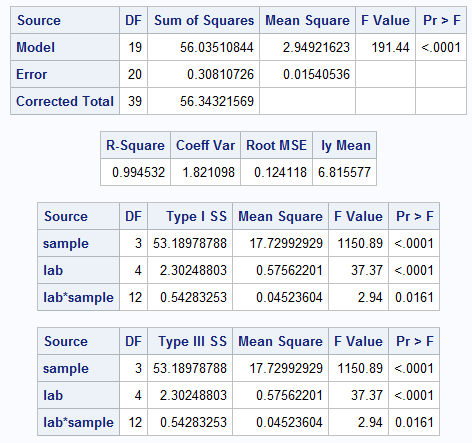
\includegraphics[scale=0.7]{MilkGLM}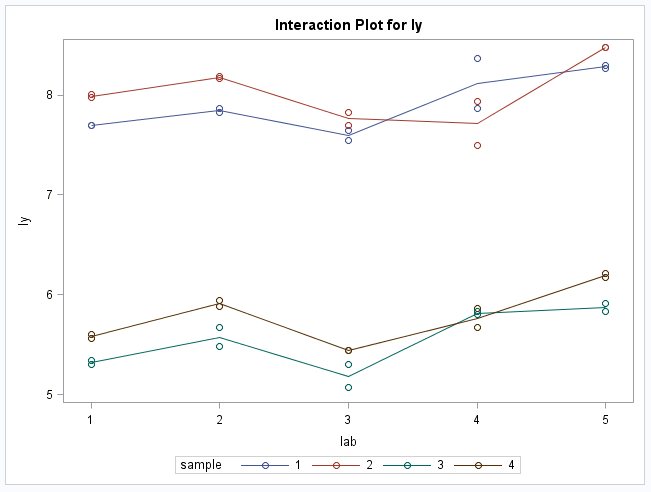
\includegraphics[scale=0.5]{MilkGLM2}
\end{center}

F-statistics divide by $MS(E)$ not appropriate error term for testing A and B main effects! \\~\\

To test for the main effect of the random factor $A$, $H_0: \sigma_A^2=0$, use the $F$-ratio $F=MS[A]/MS[AB]$.  Under $H_0$,
$F \sim F(a-1,(a-1)(b-1))=F(4,12)$, which has $F(0.05,4,12)=3.25$, yielding the $\alpha=0.05$ critical region reject $H_0$ if $F_{obs}>3.25$
The correct $F$-ratio and $p$-value for testing for random LAB (A) effect: 
$$ F=\frac{MS[A]}{MS[AB]} = \frac{0.5756}{0.0452}=12.72~~~(p=0.0003) $$
Likewise, find the correct test for the sample (B) effect. (Hint: $F(0.05,3,12)=3.49$)\\~\\%~\\~\\~\\~\\
\textcolor{red}{$$F=\frac{MS(B)}{MS(AB)}=\frac{17.75}{0.045}=391.94 > 3.49\mbox{ so Reject }H_0: \sigma^2_B=0$$}~\\~\\

Can get correct analysis in proc glm by adding in the following line:

\begin{small}
\begin{verbatim}
proc glm; class lab sample;
model ly=sample|lab;
random sample lab sample*lab; 
test h=lab sample e=sample*lab; run;
\end{verbatim}
\end{small}

\begin{center}
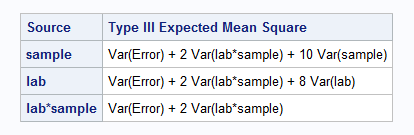
\includegraphics[scale=0.7]{MilkGLM3}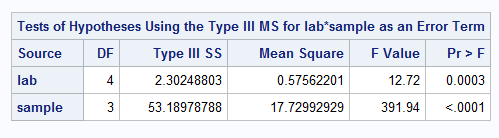
\includegraphics[scale=0.7]{MilkGLM4}
\end{center}

Now the appropriate tests are reported.  Rather than go through this, we can just use proc mixed! (see below)\\~\\

\textbf{Estimating variance components:}
The estimated variance components satisfy the following system of equations:
\begin{eqnarray*}
MS[E] & = & \hat\sigma^2 \\
MS[AB] & = & \hat\sigma^2 + n\hat\sigma_{AB}^2 \\
& = & \hat\sigma^2 + 2\hat\sigma_{AB}^2 \\
MS[A] & = & \hat\sigma^2 + nb \hat\sigma_A^2+n\hat\sigma_{AB}^2 \\
& = & \hat\sigma^2 + 8 \hat\sigma_A^2 + 2\hat\sigma_{AB}^2 \\
MS[B] & = & \hat\sigma^2 + na \hat\sigma_B^2+n\hat\sigma_{AB}^2 \\
& = & \hat\sigma^2 + 10 \hat\sigma_B^2 + 2\hat\sigma_{AB}^2 
\end{eqnarray*}
Substitution of 
\begin{eqnarray*}
MS[E] & = & 0.0154 \\
MS[AB] & = & 0.0452 \\
MS[A] & = & 0.5756 \\
MS[B] & = & 17.7299 \\
\end{eqnarray*}
into the system of equations yields the estimated variance components:
\[
\begin{array}{ccccccc}
\hat\sigma^2 &=& MS[E] &=&  &=& 0.0154 \\
\hat\sigma_{AB}^2 &=& \frac{MS[AB]-MS[E]}{n} &=&
\frac{0.0452-0.0154}{2} &=& 0.01492 \\
\hat\sigma_{A}^2 &=& \frac{MS[A]-MS[AB]}{nb} &=&
\frac{0.5756 - 0.0452}{8} &=& 0.0663 \\ 
\hat\sigma_{B}^2 &=& \frac{MS[B]-MS[AB]}{na} &=&
\frac{17.7299 - 0.0452}{10} &=& 1.768 
\end{array}\]
~\\~\\~\\
Proc mixed is our best bet for analyzing this experiment:
\begin{small}
\begin{verbatim}
proc mixed method=type3; 
class lab sample;
model ly=;
random sample|lab; 
run;
\end{verbatim}
\end{small}

\begin{center}
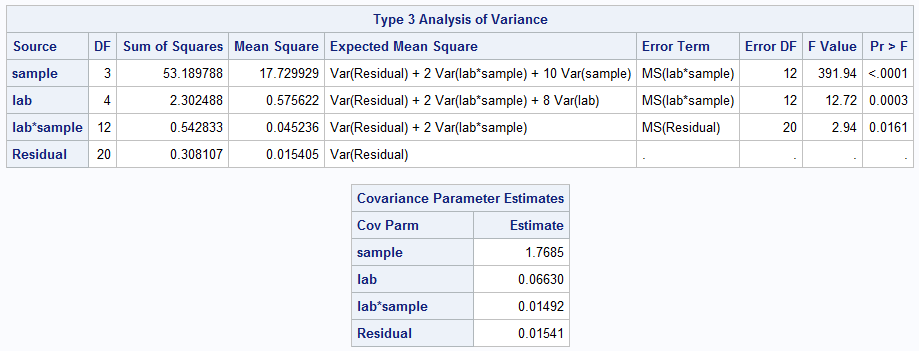
\includegraphics[scale=0.7]{MilkMixed}
\end{center}

\newpage

So, what is the conclusion from the analysis of this crossed, random effects experiment?

\begin{itemize}
\item There is evidence of variability due to laboratory$\times$sample interaction; interlaboratory effects vary by sample.
\item The estimated parameters ($\mu$ and all variance components) of the model
$$ Y_{ijk} = \mu + A_i + B_j + (AB)_{ij} + E_{ijk} $$
are
\begin{eqnarray*}
\hat\sigma^2 &=& 0.0154 \\
\hat\sigma_{AB}^2 &=&  0.0149 \\
\hat\sigma_{A}^2 &=&  0.0663 \\ 
\hat\sigma_{B}^2 &=&  1.7685  \\
\hat\mu &=&  6.82 (\mbox{log scale})
\end{eqnarray*}
\item The standard error of $\bar{Y}_{\bullet\bullet\bullet}$ can be derived by
\begin{eqnarray*}
\bar{Y}_{\bullet\bullet\bullet} &=& \mu + \bar{A}_{\bullet} + \bar{B}_{\bullet} + \overline{(AB)}_{\bullet\bullet} + \bar{E}_{\bullet\bullet\bullet} \\
\Var(\bar{Y}_{\bullet\bullet\bullet}) &=& \Var(\bar{A}_{\bullet}) + \Var(\bar{B}_{\bullet}) + \Var(\overline{(AB)}_{\bullet\bullet}) + \Var(\bar{E}_{\bullet\bullet\bullet}) \\
& = & \frac{\sigma_A^2}{a} + \frac{\sigma_B^2}{b} +  \frac{\sigma_{AB}^2}{ab} + \frac{\sigma^2}{abn} 
\end{eqnarray*}
\end{itemize}
\textbf{Estimation of standard error and approximation of $df$:}\\~\\
The standard error 
$$SE(\bar{Y}_{\bullet\bullet\bullet}) = \sqrt{\frac{\sigma_A^2}{a} + \frac{\sigma_B^2}{b} +  \frac{\sigma_{AB}^2}{ab} + \frac{\sigma^2}{abn}}$$
can be estimated by substitution of estimated variance components ($\hat\sigma^2$), which leads to 
\begin{eqnarray*}
\widehat{SE}(\bar{Y}_{\bullet\bullet\bullet}) &=& \sqrt{\frac{\hat\sigma_A^2}{a} + \frac{\hat\sigma_B^2}{b} +  \frac{\hat\sigma_{AB}^2}{ab} + \frac{\hat\sigma^2}{abn}} \\
&=& \mbox{lots of algebra and cancellations}\\
&=& \sqrt{\frac{1}{nab}\left(MS[A]+MS[B]-MS[AB]\right)}
\end{eqnarray*}
For the milk data, we have
$$ \widehat{SE}(\bar{Y}_{\bullet\bullet\bullet}) = \sqrt{\frac{1}{40}(0.58+ 17.73-0.05)} = 0.6757$$
For a $95\%$ confidence interval, we have a problem: we don't know how many $df$ are associated with a $t$ statistic based on this estimated $SE$.  \\~\\

\textbf{Satterthwaite's approximation to degrees of freedom}\\
To approximate the $df$ associated with a $t$ statistic based on a standard error of the form
$$ \sqrt{c_1 MS_1 + c_2 MS_2 + \cdots + c_k MS_k}$$
(a linear combination of mean square terms), use the \textbf{Satterthwaite approximation:}
$$ \widehat{df} = \frac{(c_1 MS_1 + c_2 MS_2 + \cdots + c_k MS_k)^2}{(c_1 MS_1)^2/df_1 + (c_2 MS_2)^2/df_2 + \cdots + (c_k MS_k)^2/df_k}$$
The degrees of freedom associated with $\widehat{SE}(\bar{Y}_{\bullet\bullet\bullet})$ is approximated by
$$\widehat{df} = \frac{(0.6757)^4}{(\frac{1}{40}17.73)^2/3 + (\frac{1}{40}0.58)^2/4 +  (\frac{1}{40}0.045)^2/12} = 3.18$$
Using $t(0.025,3.18) = 3.08$, a $95\%$ confidence interval for the (log) mean $\mu$ among the population of all labs and samples is given by
$$ 6.82 \pm 3.08 (0.6757)= 6.82 \pm 2.08$$

In proc mixed we can get this using:
\begin{small}
\begin{verbatim}
proc mixed cl method=type3; 
   class sample lab;
   model ly=/ddfm=satterth cl;
   random sample|lab;
run;
\end{verbatim}
\end{small}

\begin{center}
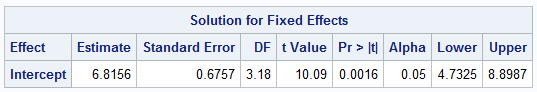
\includegraphics[scale=0.7]{MilkMixed2}
\end{center}

\newpage

\textbf{More Two-factor mixed models analysis examples}
\begin{itemize}
\item Recall the Campylobacter count chicken experiment:
\begin{itemize}
\item Crossed design with two factors
\begin{itemize}
\item Location (4 levels)
\item Day (3 levels)
\end{itemize}
\item $n=10$ chickens per combo for a total of $N=120$ observations
\item Location of measurement is fixed, Day is random and the factors are crossed ($4 \times 3$ layout)
\end{itemize}
\end{itemize}

Recall:  Model being fit is 
$$Y_{ijk} = \mu + \alpha_i + B_j + (\alpha B)_{ij} + E_{ijk}$$
with variance components $\sigma_B^2, \sigma_{\alpha B}^2, \sigma^2$.\\~\\
Fixed Factor A: location \\
Random Factor B: day\\~\\

The Mixed model from previous was fit to this data using the code:\\
\begin{small}
\begin{verbatim}
proc mixed data=bashor method=type3 plots=all;
class day location;
model ly=location; *ly=log(y) was used as non-constant variance was evident when using y as response
random day day*location;
lsmeans location/adjust=tukey cl;
run;
\end{verbatim}
\end{small}

\begin{center}
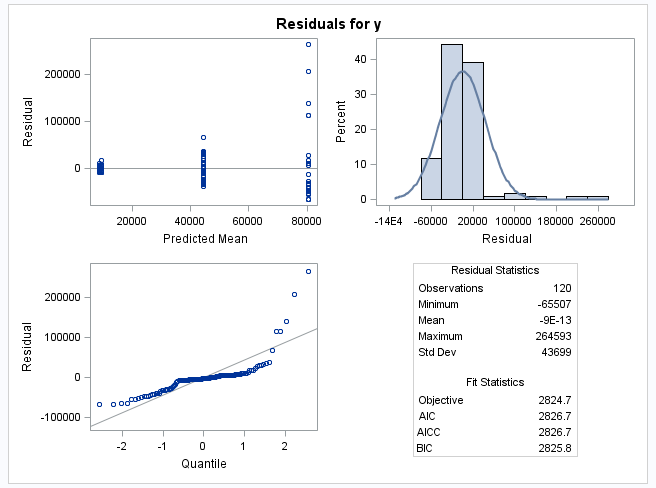
\includegraphics[scale=0.7]{Campy1}\\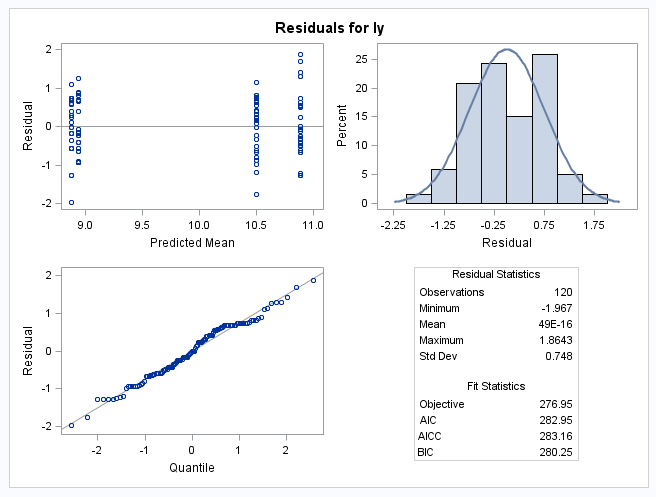
\includegraphics[scale=0.7]{Campy2}
\end{center}

First plot = residual plot using $y$ as response, second plot = residual plot using $log(y)$ as response.  (Note: would also check conditional residuals.)

\begin{center}
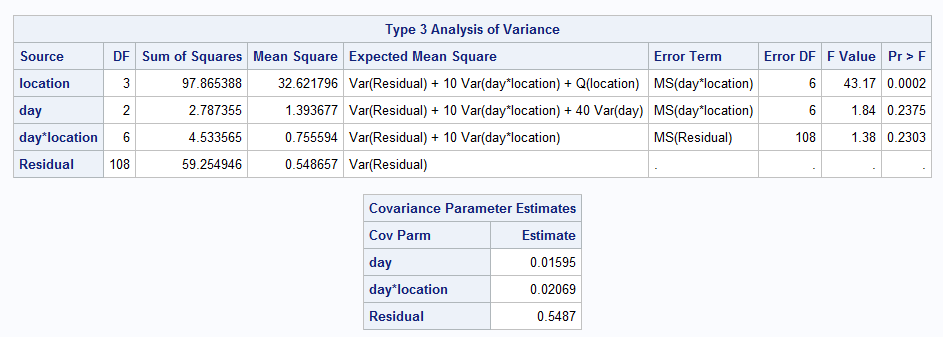
\includegraphics[scale=0.7]{Campy3}\\
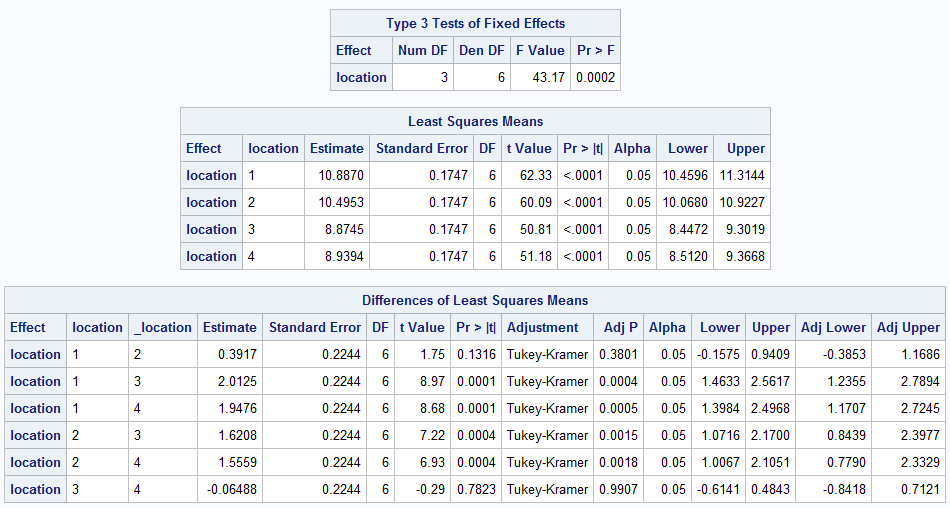
\includegraphics[scale=0.7]{Campy5}\\
\end{center}

Output from model above.  Below is the interaction plot (found using proc glm).

\begin{center}
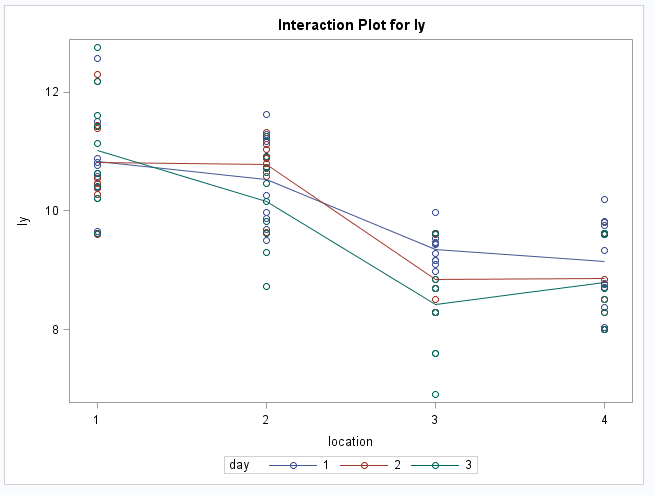
\includegraphics[scale=0.7]{Campy4}
\end{center}

In the model we estimate the variance components by:
\begin{eqnarray*}
\hat\sigma^2 & = & MS[E]  =  0.55 \\
\hat\sigma_{\alpha B}^2 & = & \frac{MS[AB]-MS[E]}{n} \\
& = & \frac{0.76-0.55}{10}  =  0.021  \\
\hat\sigma_{B}^2 & = & \frac{MS[B]-MS[AB]}{na} \\
& = & \frac{1.39-0.76}{40}  =  0.016
\end{eqnarray*}

To test $H_0: \sigma_{\alpha B}^2=0$, use 
$$F_{AB}=\frac{MS[AB]}{MS[E]}=\frac{0.76}{0.55}=1.38$$
on $(a-1)(b-1)=6$ and $ab(n-1)=108$ $df$.  The $p$-value is $0.2303$, providing no evidence of a random day $\times$ location interaction effect. \\~\\
The variance component for this random effect is estimated by 0.021.  Intepretation: Since we failed to reject, there is no evidence that day-to-day variability varies by location.  The estimated variance component is itself very small.\\~\\

\textbf{Implied correlation structure}\\
What is the correlation of two observations taken on the same day 
\begin{itemize}
\item at the same location? \textcolor{red}{same location, same day}
\item at different locations? \textcolor{red}{different location, same day}
\end{itemize}

Recall that $Y_{ijk}=\mu + \alpha_i + B_j + (\alpha B)_{ij} +E_{ijk}$.
\begin{eqnarray*}
Corr(Y_{ij k_1},Y_{ij k_2}) & = & \frac{\Cov(Y_{ij k_1},Y_{ij k_2})} 
{\sigma^2 + \sigma_{B}^2 + \sigma_{\alpha B}^2}\\
& = & \frac{\Cov(B_j,B_j) + \Cov((\alpha B)_{ij}, (\alpha B)_{ij})}
{\sigma^2 + \sigma_{B}^2 + \sigma_{\alpha B}^2}\\
& = & \frac{\sigma_B^2 + \sigma_{\alpha B}^2}
{\sigma^2 + \sigma_{B}^2 + \sigma_{\alpha B}^2}\\
Corr(Y_{1 j k_1},Y_{2j k_2}) & = & \frac{\Cov(Y_{1j k_1},Y_{2j k_2})} 
{\sigma^2 + \sigma_{B}^2 + \sigma_{\alpha B}^2}\\
& = & \frac{\Cov(B_j,B_j)} 
{\sigma^2 + \sigma_{B}^2 + \sigma_{\alpha B}^2}\\
& = & \frac{\sigma_B^2} 
{\sigma^2 + \sigma_{B}^2 + \sigma_{\alpha B}^2}\\
\end{eqnarray*}
Estimates of these correlations are 
\begin{itemize}
\item $\frac{0.016+0.021}{0.016 + 0.021 + 0.55} = \frac{0.037}{.587} = 0.063$
\item $\frac{0.016}{0.016 + 0.021 + 0.55} = \frac{0.016}{.587} = 0.027$
\end{itemize}
~\\~\\~\\~\\
\textbf{Some analysis of fixed effects}\\
Consider testing for a fixed effect of location.  That is, test the hypothesis that average bacteria counts are constant across the locations, \\~\\~\\
$$ F_A = \frac{MS[A]}{MS[AB]} = \frac{32.6}{0.76} = 43.2$$
on $a-1=3$ and $(a-1)(b-1)=6$ $df$, which is significant ($p=0.0002$).\\~\\
Since significant fixed effect, we want to estimate the pairwise comparisons among location means, such as, $\alpha_4-\alpha_3$, consider
$$\hat\theta=\bar{y}_{4\bullet\bullet}-\bar{y}_{3\bullet\bullet} = 8.940-8.875 = - 0.065$$
Note that 
$$ \Var(\bar{Y}_{4\bullet\bullet}-\bar{Y}_{3\bullet\bullet}) \neq \sigma^2(\frac{1}{nb} + \frac{1}{nb})$$
Since our $Y$'s are not independent anymore!\\~\\
What is $SE(\hat\theta)$ and how can it be estimated?
\begin{eqnarray*}
\hat\theta &=& \bar{Y}_{4\bullet\bullet}-\bar{Y}_{3\bullet\bullet} \\
&=&\mu+\alpha_4 + \bar{B}_{\bullet} + \overline{\alpha B}_{4\bullet} + \overline{E}_{4\bullet\bullet} -(\mu+\alpha_3 + \bar{B}_{\bullet} + \overline{\alpha B}_{3\bullet} + \overline{E}_{3\bullet\bullet}) \\
&=& \alpha_4 -\alpha_3 + \overline{\alpha B}_{4\bullet} - \overline{\alpha B}_{3\bullet} + \overline{E}_{4\bullet\bullet} - \overline{E}_{3\bullet\bullet} 
\end{eqnarray*} 
which has variance
\begin{eqnarray*} 
\Var(\hat\theta)&=& \Var(\overline{\alpha B}_{4\bullet}) + \Var(\overline{\alpha B}_{3\bullet}) 
+ \Var(\overline{E}_{4\bullet\bullet}) + \Var(\overline{E}_{3\bullet\bullet}) \\ 
 &=& 2 \frac{\sigma_{\alpha B}^2}{b} + 2 \frac{\sigma^2}{nb} \\
 &=& \frac{2}{nb} (\sigma^2 + n \sigma_{\alpha B}^2)
\end{eqnarray*} 
which can be estimated nicely on $(a-1)(b-1)=6~df$ by
$$\hat{\Var}(\hat\theta) = \frac{2}{nb} MS[AB]$$
for the chickens, where $\overline{y}_{4\bullet\bullet} - \overline{y}_{3\bullet\bullet}=-0.06$ the $SE$ is
$$\sqrt{\widehat{\Var}(\hat\theta)} = \sqrt{\frac{2}{3*10} 0.76} = 0.22$$
Since $t(0.025,6) =2.45$, a $95\%$ c.i. for $\theta$ given by $-0.06 \pm 2.45(0.22)$.\\~\\
Reporting standard errors for sample means of levels of fixed factor, like LOCATION means, is a little messier:
\begin{eqnarray*}
\overline{Y}_{i\bullet\bullet} &= \mu + & \alpha_i + \overline{B}_{\bullet} + \overline{\alpha B}_{i\bullet} + \overline{E}_{i\bullet\bullet} \\
\Var(\overline{Y}_{i\bullet\bullet}) &=& \Var(\overline{B}_{\bullet}) + \Var(\overline{\alpha B}_{i\bullet}) + \Var(\overline{E}_{i\bullet\bullet}) \\
& = & \frac{\sigma_B^2}{b} + \frac{\sigma_{\alpha B}^2}{b} + \frac{\sigma^2}{nb} \\
& = & \frac{1}{nb}(n\sigma_B^2 + n \sigma_{\alpha B}^2 + \sigma^2)\\
& & \mbox{ estimated by } \\
\widehat{\Var}(\overline{Y}_{i\bullet\bullet}) &=& 
\frac{1}{nb}(n\hat\sigma_B^2 + n \hat\sigma_{\alpha B}^2 + \hat\sigma^2) \\
& = & \mbox{ algebra yields a linear combo of multiple EMS terms} \\
& = & \frac{1}{nab}\{(a-1)MS[AB] + MS[B]\}
\end{eqnarray*}
The standard error is estimated easily enough:
\begin{eqnarray*}
\widehat{SE}(\overline{Y_{i\bullet\bullet}}) & = & \sqrt{\frac{1}{nab}\{(a-1)MS[AB] + MS[B]\}} \\
%&=& \sqrt{\frac{1}{16}\{(2-1)61.6 + 143.8\}} \\
&=& \sqrt{\frac{1}{120}\{(4-1)0.76 + 1.39\}} \\
& = & \sqrt{0.03} = 0.175
\end{eqnarray*}
but the $df$ must be approximated using the Satterthwaite approach
$$ \hat{df} = \frac{0.175^4}{\frac{1}{120^2}\left(\frac{((4-1)0.76)^2}{6} + 
\frac{1.39^2}{2}\right)} = 7.33 $$
with $df_{AB}=6,df_{B}=2$.  Since $t(0.025,7.33)=2.34$, a $95\%$ c.i.  for
the population mean of location 1, for example, is $10.9 \pm 2.34 (0.175)$.

\newpage

\textbf{SAS code to fit two-factor random effects model for plant acid data}:\\
Recall:  Both effects are random and leaf is nested in plant (since leaf 1 from plant 2 doesn't really mean the same as leaf 1 from plant 2).

$$Y_{ijk} = \mu + A_i + B_{j(i)} + E_{ijk}$$
w/ variance components $\sigma^2,\sigma_A^2,\sigma_{B(A)}^2$.\\

\begin{small}
\begin{verbatim}
proc mixed method=type3 cl;
class plant leaf;
model y=/cl;
random plant leaf(plant);
run;
\end{verbatim}
\end{small}

\begin{center}
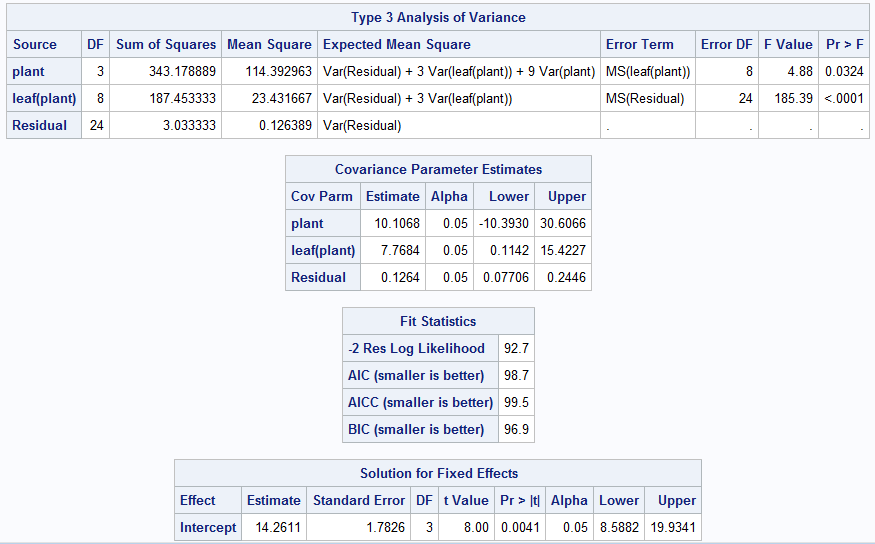
\includegraphics[scale=0.7]{Plant}
\end{center}

Variance components estimated as
\begin{eqnarray*}
\hat\sigma^2 & = & MS[E]  =  0.13 \\
\hat\sigma_{B(A)}^2 & = & \frac{MS[B(A)]-MS[E]}{n} \\
& = & \frac{23.4-0.13}{3}  =  7.8  \\
\hat\sigma_{A}^2 & = & \frac{MS[A]-MS[B(A)]}{nb} \\
& = & \frac{114.4-23.4}{9}  =  10.1
\end{eqnarray*}
~\\
To test for random effect of nested factor $B$ (leaf), $H_0: \sigma_{B(A)}^2=0$,
$$ F=\frac{MS[B(A)]}{MS[E]}=\frac{23.4}{0.13}=185.4$$ 
on $(b-1)a=8$ and $(n-1)ab=24$ df  ($p$-value $<0.0001$).\\~\\

To test for random effect of factor $A$ (plant), $H_0: \sigma_A^2=0$, 
$$ F=\frac{MS[A]}{MS[B(A)]} = \frac{114.4}{23.4} = 4.88$$
on $a-1=3$ and $(b-1)a=8 df$ with $p=0.0324$.   \\~\\

So there is evidence of both a random plant effect and a random leaf effect, nested in plant.  The magnitudes of these effects are quantified by the estimated variance components.  The statistical significance addressed by the $p$-values.  \\~\\~\\

\textbf{Implied correlation structure for plant acids:}\\
What is the correlation of two observations taken from the same plant
\begin{itemize}
\item and the same leaf?
\item and different leaves?
\end{itemize}
Recall that $Y_{ijk}=\mu + A_i + B_{j(i)} + E_{ijk}$.
\begin{eqnarray*}
Corr(Y_{ij k_1},Y_{ij k_2}) & = & \frac{\Cov(Y_{ij k_1},Y_{ij k_2})} 
{\sigma^2 + \sigma_{A}^2 + \sigma_{B(A)}^2}\\
& = & \frac{\Cov(A_i,A_i) + \Cov(B_{j(i)}, B_{j(i)})}
{\sigma^2 + \sigma_{A}^2 + \sigma_{B(A)}^2}\\
& = & \frac{\sigma_A^2 + \sigma_{B(A)}^2}
{\sigma^2 + \sigma_{A}^2 + \sigma_{B(A)}^2}\\
Corr(Y_{i j_1 k_1},Y_{i j_2 k_2}) & = & \frac{\Cov(Y_{i j_1 k_1},Y_{2 j_2 k_2})} 
{\sigma^2 + \sigma_{A}^2 + \sigma_{B(A)}^2}\\
& = & \frac{\Cov(A_i,A_i)} 
{\sigma^2 + \sigma_{A}^2 + \sigma_{B(A)}^2}\\
& = & \frac{\sigma_A^2} 
{\sigma^2 + \sigma_{A}^2 + \sigma_{B(A)}^2}\\
\end{eqnarray*}
Estimates of these correlations are 
\begin{itemize}
\item $\frac{10.1+7.8}{10.1+7.8+0.13} = \frac{17.9}{18.0} = 0.99$
\item $\frac{10.1}{10.1+7.8+0.13} = \frac{10.1}{18.0} = 0.56$
\end{itemize}
This means that two measurements taken on the same leaf are almost perfectly correlated.  Almost all the variation in any measurement can be
explained by the leaf and plant effects.

\newpage

\textbf{Experiment with light treatments on seedlings:}\\
Recall we have a fixed treatment effect with a nested random effect.  
\begin{itemize}
\item Response ($y$) is seedling height, 
\item treatments are light sources, intensities,
\item experimental units are 10 pots (points on graph).
\end{itemize}
Model to fit
$$ Y_{ijk} = \mu + \alpha_i + P_{(i)j} + E_{ijk} $$
$\alpha_i$ - treatment effects for $i=1,2,3,4,5$ \\
$P_{(i)j}$ - pot effects, nested in treatments, $j=1,2$ for each $i$. \\
$E_{ijk}$ -  seedling/experimental errors, $k=1,2$
$$P_{(i)j} \iid N(0,\sigma_P^2), \ \ \ E_{ijk} \iid N(0,\sigma^2) \ \ (P_{(i)j} \perp E_{ijk})$$

\begin{small}
\begin{center}
\begin{tabular}{cc|cc}
Treatment & Pot & Seedling 1 & Seedling 2 \\ \hline
1          &       1       &      32.94      &      35.98 \\
1          &       2       &      34.76      &      32.40 \\
2          &       1       &      30.55      &      32.64 \\
2          &       2       &      32.37      &      32.04 \\
3          &       1       &      31.23      &      31.09 \\
3          &       2       &      30.62      &      30.42 \\
4          &       1       &      34.41      &      34.88 \\
4          &       2       &      34.07      &      33.87 \\
5          &       1       &      35.61      &      35.00 \\
5          &       2       &      33.65      &      32.91 \\ \hline
\end{tabular}
\end{center}
\end{small}
~\\
SAS code for fitting this mixed model is given below:\\
	
\begin{small}
\begin{verbatim}
proc mixed data=plantheight method=type3;
class treatment pot;
model height=treatment;
random pot(treatment);
lsmeans treatment/adjust=tukey cl;
run;
\end{verbatim}
\end{small}

\begin{center}
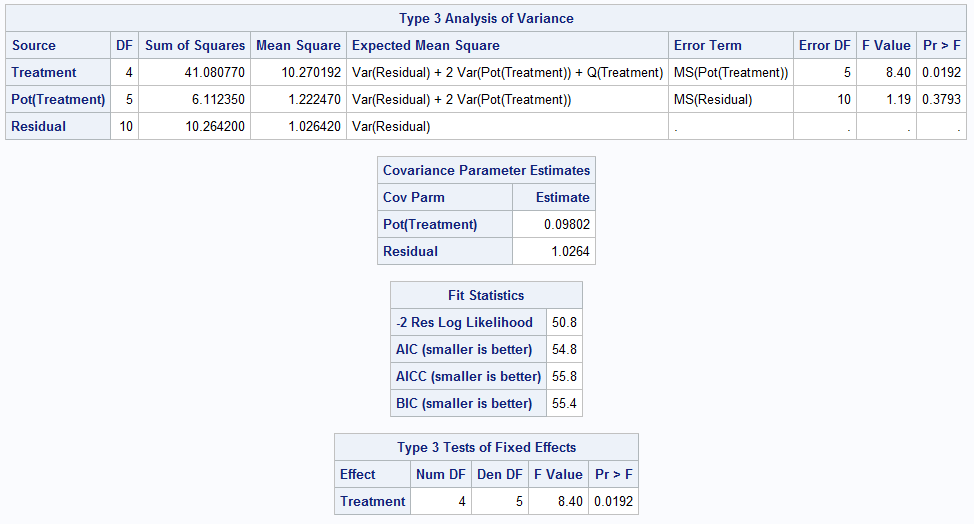
\includegraphics[scale=0.7]{Heights}\\
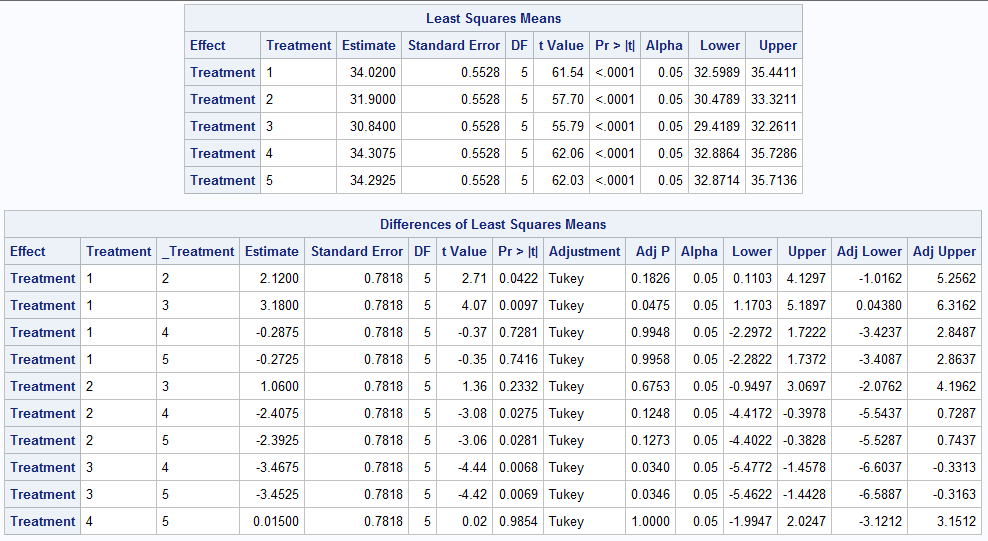
\includegraphics[scale=0.7]{Heights2}
\end{center}

\newpage

For treatment effects, use $MS(Pot(treatments))$ as error term.  \\
For example, for $H_0: \alpha_1=\alpha_2=\cdots=0$, use
$$ F = \frac{MS(\mbox{treatment})}{MS(\mbox{Pot(treatment)})} \sim F_{5-1,5(2-1)} \mbox{ or }F_{4,5}$$
Be careful not to use
$$ F = \frac{MS(\mbox{treatment})}{MS(E)}$$
For these data, we get
$$ F=\frac{10.27}{1.22}=8.4 (df=4,5, p=.0192)$$
providing evidence of a treatment effect on plant heights.
